\label{chap:map}
A partir do levantamento dos pressupostos pedagógicos das diferentes propostas de avaliação, realizado no \refCap{chap:ref} e da catalogação das ferramentas de avaliação, disponíveis no \refCap{chap:ava}, foi possível mapear as ferramentas que podem estar vinculadas a uma ou a outra avaliação. Para cada ferramenta do catálogo, podemos identificar as características descritas de cada tipo de avaliação e, posteriormente, estruturar uma matriz com este mapeamento. A \refFig{fig:passos} ilustra o processo de mapeamento proposto.
\\
\begin{figure}[h]
    \centering
\tikzset{
    mynode/.style={
        draw, rectangle, align=center, text width=5cm, font=\small, inner sep=1ex},
    mylabel/.style={
        draw, rectangle, align=center, rounded corners, font=\small\bf, inner sep=1ex, 
        fill=cyan!30, minimum height=3cm},
    arrow/.style={
        very thick,->,>=stealth}
}

\begin{tikzpicture}[
    node distance=1.5cm,
    start chain=1 going below,
    every join/.style=arrow,
    ]
    % the chain in the center going below
    \coordinate[on chain=1] (tc);
    \node[mynode, on chain=1] (n2)
        {Estabelecimento da relação\\entre (Y)x(W)};
    \node[mynode, join, on chain=1] (n3)
        {Estruturação do mapeamento em uma matriz de associação};

    % the nodes at the top  
    \node[mynode, left=1cm of tc, anchor=south east] (n1l)
        {Levantamento dos tipos\\ de avaliação (Y)};
    \node[mynode, right=1cm of tc, anchor=south west] (n1r) 
        {Catalogação das ferramentas avaliativas (W)};

    \coordinate (n2nl) at ([xshift=-2cm]n2.north);
    \coordinate (n2nr) at ([xshift= 2cm]n2.north);
    \draw[arrow] (n1l.south -| n2nl) -- (n2nl);
    \draw[arrow] (n1r.south -| n2nr) -- (n2nr);

    % the labels on the left
    \begin{scope}[start chain=going below, xshift=-8cm, node distance=.8cm]
        \node[mylabel, on chain] {\rotatebox{90}{Identificação}};
        \node[mylabel, on chain] {\rotatebox{90}{Mapeamento}};
    \end{scope}

    % the title
    \node[above=2cm of tc, font=\bf] {Processo de Mapeamento};
\end{tikzpicture}
    \caption{Passos do mapeamento.}
    \label{fig:passos}
\end{figure}

\textbf{--> NÃO PODES terminar uma seção com imagem. Tens que finalizar com um texto que faz um link com a seção seguinte.}
%%%%%%%%%%%%%%%%%%%%%%%%%%%%%%%%%%%%%%%%%%%%%%%%%%%
%%%%%%%%%%%%%%%%%%%%%%%%%%%%%%%%%%%%%%%%%%%%%%%%%%%
%%%%%%%%%%%%%%%%%%%%%%%%%%%%%%%%%%%%%%%%%%%%%%%%%%%
%%%%%%%%%%%%%%%%%%%%%%%%%%%%%%%%%%%%%%%%%%%%%%%%%%%

\section{Relação entre ferramentas e avaliação}

Para estabelecer a relação entre uma ferramenta (W) e um tipo de avaliação (Y), houve a necessidade de se responder à seguinte pergunta: qual a potencial aplicabilidade da ferramenta na categoria de avaliação investigada?

Cada ferramenta de avaliação teve seu grau de aplicabilidade inspecionado em relação a cada um dos pressupostos pedagógicos apresentados no Organograma da \refFig{fig:organogfunc}. As possíveis respostas foram parametrizadas conforme abaixo:

\begin{itemize}
    \item Aplicável, quando a avaliação descreve propriamente o uso da funcionalidade da ferramenta, considerando-se seus requisitos. O símbolo ``\ding{108}'' foi utilizado para representar graficamente a resposta.
    \item Parcialmente aplicável, quando a avaliação descreve parte da funcionalidade. O símbolo ``\ding{115}'' representa a resposta. \item Não aplicável, quando a avaliação não descreve o uso da funcionalidade. O símbolo ``\ding{53}'' representa a resposta. 
\end{itemize}

Considerando os parâmetros definidos, a ferramenta ``Acompanhar questionário'' quando analisada sob o aspecto da formalização, foi classificada como aplicável quanto à utilização como avaliação formal, e como parcialmente aplicável na avaliação informal. Isso porque ela atua com ferramentas formais de aprendizagem como questionários. E também porque fornece dados estatísticos capazes de fornecer uma avaliação informal ao docente sobre seu uso.

\textbf{--> ESTE TRECHO está bastante confuso... Recomendo reescrever. Tens que fazer referência à imagem onde estao as ferramentas 3.4}

Do mesmo modo, a aplicabilidade de cada ferramenta de avaliação foi verificada quanto ao aspecto da formalização. Os resultados completos para cada item da lista de ferramentas são apresentados na \refTab{tab:tabrelYxW}. A partir desta representação, pode-se verificar que o aspecto da formalização é aplicável em pelo menos um das dois subtipos. Ou seja, uma avaliação pode ser formal ou informal e, em alguns casos, formal e informal. Mas em nenhum caso a classificação foi dispensada. O que faz todo o sentido, já que os aspectos são considerados como necessários para configurar uma avaliação.

\bigskip
\begin{table}[h]
\setlength{\bigstrutjot}{3pt}
\settowidth\rotheadsize{long text}
\caption{Lista da Relação (Y)x(W)}
\label{tab:tabrelYxW}
\centering
\begin{tabular}{|l|c|c|}
\addlinespace \hline
    \bigstrut \textbf{Ferramentas}  & \multicolumn{2}{c|}{Formalização}\\
\cline{2-3}
    \bigstrut
    \textbf{de avaliação}  & Formal & Informal \\
\hline
    \bigstrut[t]
    Gerenciamento de grupo	& \ding{108} & \ding{115}\\ \hline
    Programação do curso    & \ding{108}  & \ding{53}\\ \hline
    Acompanhar anúncios     & \ding{53} & \ding{108}\\ \hline
    Acompanhar notificações & \ding{53} & \ding{108}\\ \hline
    Recuperação de conteúdo & \ding{53} & \ding{108}\\ \hline
    Map. de Competências    & \ding{53} & \ding{108}\\ \hline
    Acompanhar colaboração  & \ding{115} & \ding{108}\\ \hline
    Acompanhar dificuldades & \ding{53} & \ding{108}\\ \hline
    Acompanhar questionários & \ding{108} & \ding{115}\\ \hline
    Revisão de textos       & \ding{108}  & \ding{53}\\ \hline 
    Acompanhar tarefas      & \ding{108}  & \ding{53}\\ \hline  
    Acompanhar aulas        & \ding{53} & \ding{108}\\ \hline
    Acompanhar exames       & \ding{108}  & \ding{53}\\ \hline  
    Registrar notas         & \ding{108}  & \ding{53}\\ \hline 
    Acompanhar notas/feedback  & \ding{53} & \ding{108}\\ \hline 
    Orientação              & \ding{108}  & \ding{53}\\ \hline        
    \bigstrut[b]
    Moderação               & \ding{108}  & \ding{53}\\  
\hline
\end{tabular}
\end{table}
\bigskip

%%%%%%%%%%%%%%%%%%%%%%%%%%%%%%%%%%%%%%%%%%%%%%%%%%%
%%%%%%%%%%%%%%%%%%%%%%%%%%%%%%%%%%%%%%%%%%%%%%%%%%%
%%%%%%%%%%%%%%%%%%%%%%%%%%%%%%%%%%%%%%%%%%%%%%%%%%%
%%%%%%%%%%%%%%%%%%%%%%%%%%%%%%%%%%%%%%%%%%%%%%%%%%%

\section{Matriz de ferramentas e avaliações}%

\textbf{-->não utilizar penúltimo, acima, abaixo, ao lado... - somente referenciar a imagem que representa. Recomendo reescrever pois está muito coloquial, quase parecendo um passo a passo informal.}
Ao continuarmos empregando a questão da aplicabilidade em cada aspecto do penúltimo nível do Organograma das funções de avaliação, representado pela \refFig{fig:organogfunc}, chegaremos em um mapeamento de todas as ferramentas de avaliação em relação a todos os aspectos avaliativos encontrados. A \refTab{tab:matrizYxW} exibe os resultados completos da matriz.

Com isso, podemos verificar não apenas quais ferramentes de avaliação são indicadas para a condução de uma avaliação diagnóstica, defendida por Luckesi\textbf{ (REFERÊNCIA?)}, mas também podemos vincular essa avaliação com as ferramentas que de alguma forma precisariam estar disponíveis aos alunos para que esse objetivo seja alcançado, ao utilizar conjuntamente a matriz de vínculos apresentada na \refFig{fig:ferramentas}.


%\begin{landscape}

\begin{table}[ht!]
\setlength{\bigstrutjot}{4pt}
\settowidth\rotheadsize{Valores e atitudes}
\caption{Matriz relacional entre as ferramentas de avaliação e funções de avaliação.}
\label{tab:matrizYxW}
\centering
\resizebox{\textwidth}{!}{%
\begin{tabular}{|l|c|c|c|c|c|c|c|c|c|c|c|c|c|c|c|}
\addlinespace \hline
    \bigstrut &
        \multicolumn{2}{c|}{\cellcolor{blue!25}forma} & \multicolumn{3}{c|}{\cellcolor{red!25}composição} & \multicolumn{2}{c|}{\cellcolor{green!25}freq.} & \multicolumn{3}{c|}{\cellcolor{uclagold!25}função} & \multicolumn{3}{c|}{\cellcolor{purple!25}objeto} & \multicolumn{2}{c|}{\cellcolor{cyan!25}espaço}\\
        \cline{2-3} \cline{4-6} \cline{7-8} \cline{9-11} \cline{12-14} \cline{15-16}
    \bigstrut
    \textbf{Ferramentas de avaliação}  & \rothead{Formal} & \rothead{Informal} & \rothead{Instrucional} & \rothead{Comportamental} & \rothead{Valores e atitudes} & \rothead{Pontual} & \rothead{Contínua} & \rothead{Somativa} & \rothead{Diagnóstica} & \rothead{Formativa} & \rothead{Aluno} & \rothead{Disciplina} & \rothead{Equipe} & \rothead{Plataforma} & \rothead{App de terceiros}\\
\hline
    \bigstrut[t]
    
    Geren. de grupo	&\ding{108}&\ding{115}&\ding{108} &\ding{108}&\ding{53}&\ding{53}&\ding{108}&\ding{53}&\ding{115}
    &\ding{108}&\ding{108}&\ding{53}&\ding{108}&\ding{108}&\ding{53}\\ 
    \hline
    Programação do curso &\ding{108}&\ding{53}&\ding{53} &\ding{53}&\ding{53}&\ding{53}&\ding{108}&\ding{53}&\ding{53}
    &\ding{108}&\ding{53}&\ding{108}&\ding{53}&\ding{108}&\ding{53}\\ 
    \hline 
    Acompanhar anúncios &\ding{53}&\ding{108}&\ding{108} &\ding{108}&\ding{53}&\ding{108}&\ding{53}&\ding{53}&\ding{108}
    &\ding{53}&\ding{108}&\ding{53}&\ding{53}&\ding{108}&\ding{53}\\ 
    \hline
    Acomp. notificações &\ding{53}&\ding{108}&\ding{53} &\ding{108}&\ding{53}&\ding{108}&\ding{53}&\ding{53}&\ding{108}
    &\ding{53}&\ding{108}&\ding{53}&\ding{53}&\ding{108}&\ding{53}\\ 
    \hline 
    Recup. de conteúdo &\ding{53}&\ding{108}&\ding{53} &\ding{108}&\ding{53}&\ding{53}&\ding{108}&\ding{53}&\ding{108}
    &\ding{53}&\ding{108}&\ding{115}&\ding{53}&\ding{108}&\ding{115}\\ 
    \hline
    Map. de Competências &\ding{53}&\ding{108}&\ding{53} &\ding{108}&\ding{115}&\ding{53}&\ding{108}&\ding{53}&\ding{108}
    &\ding{108}&\ding{108}&\ding{53}&\ding{115}&\ding{108}&\ding{53}\\ 
    \hline 
    Acomp. colaboração  &\ding{115}&\ding{108}&\ding{115} &\ding{108}&\ding{115}&\ding{53}&\ding{108}&\ding{115}&\ding{108}
    &\ding{108}&\ding{108}&\ding{53}&\ding{108}&\ding{108}&\ding{53}\\ 
    \hline
    Acomp. dificuldades &\ding{53}&\ding{108}&\ding{108} &\ding{115}&\ding{53}&\ding{53}&\ding{108}&\ding{53}&\ding{108}
    &\ding{108}&\ding{108}&\ding{115}&\ding{53}&\ding{108}&\ding{53}\\ 
    \hline 
    Acomp. questionários &\ding{108}&\ding{115}&\ding{108} &\ding{115}&\ding{53}&\ding{53}&\ding{108}&\ding{115}&\ding{115}
    &\ding{108}&\ding{108}&\ding{115}&\ding{53}&\ding{108}&\ding{53}\\ 
    \hline
    Revisão de textos &\ding{108}&\ding{53}&\ding{108} &\ding{53}&\ding{115}&\ding{53}&\ding{108}&\ding{108}&\ding{115}
    &\ding{115}&\ding{108}&\ding{53}&\ding{53}&\ding{108}&\ding{115}\\ 
    \hline 
    Acompanhar tarefas &\ding{108}&\ding{53}&\ding{108} &\ding{115}&\ding{53}&\ding{53}&\ding{108}&\ding{108}&\ding{115}
    &\ding{108}&\ding{108}&\ding{115}&\ding{53}&\ding{108}&\ding{115}\\ 
    \hline  
    Acompanhar aulas &\ding{53}&\ding{108}&\ding{53} &\ding{108}&\ding{53}&\ding{53}&\ding{108}&\ding{53}&\ding{108}
    &\ding{53}&\ding{108}&\ding{108}&\ding{53}&\ding{108}&\ding{115}\\ 
    \hline 
    Acompanhar exames &\ding{108}&\ding{53}&\ding{108} &\ding{115}&\ding{115}&\ding{53}&\ding{108}&\ding{108}&\ding{115}
    &\ding{53}&\ding{108}&\ding{115}&\ding{53}&\ding{108}&\ding{115}\\ 
    \hline  
    Registrar notas &\ding{108}&\ding{53}&\ding{108} &\ding{53}&\ding{53}&\ding{53}&\ding{108}&\ding{108}&\ding{53}
    &\ding{53}&\ding{108}&\ding{53}&\ding{53}&\ding{108}&\ding{53}\\ 
    \hline 
    Acomp. notas/feedback &\ding{53}&\ding{108}&\ding{108} &\ding{108}&\ding{53}&\ding{53}&\ding{108}&\ding{53}&\ding{108}
    &\ding{115}&\ding{108}&\ding{53}&\ding{53}&\ding{108}&\ding{53}\\ 
    \hline 
    Orientação &\ding{108}&\ding{53}&\ding{115} &\ding{115}&\ding{53}&\ding{53}&\ding{108}&\ding{53}&\ding{115}
    &\ding{108}&\ding{108}&\ding{53}&\ding{108}&\ding{108}&\ding{53}\\ \hline        
    \bigstrut[b]
    
    Moderação &\ding{108}&\ding{53}&\ding{53} &\ding{108}&\ding{108}&\ding{108}&\ding{53}&\ding{53}&\ding{115}
    &\ding{108}&\ding{108}&\ding{53}&\ding{108}&\ding{108}&\ding{53}\\  
\hline
\end{tabular}}
    \begin{tablenotes}
      \small
      \item Legenda: \ding{108} Aplicável; \ding{115} Parcialmente aplicável; \ding{53} Não aplicável.
    \end{tablenotes}
\end{table}
\bigskip


%\end{landscape}

%\begin{figure}[h]
%    \centering
%        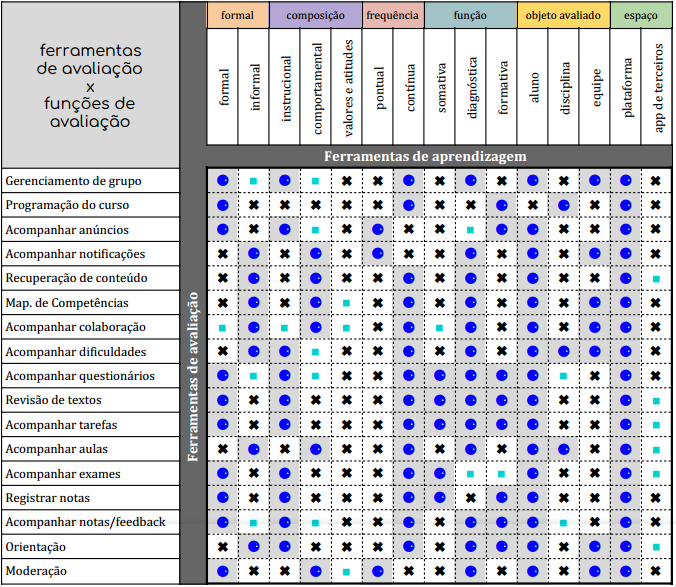
\includegraphics[width=\textwidth]{img/avaliacao_funcoes.png}
%    \caption{Relação entre ferramentas de avaliação e funções de avaliação.}
%    \label{fig:funcoes}
%\end{figure}